% Friction-Cliff-Bench technical report.
% Build: cd paper && tectonic main.tex
% Every number in a results section is \input from files that scripts/make_figures.py and
% scripts/grounding_comma.py generate from the raw run logs (rule: no numbers without N and a CI).
\documentclass[11pt]{article}
\usepackage[margin=1in]{geometry}
\usepackage{amsmath,amssymb}
\usepackage{graphicx}
\usepackage{booktabs}
\usepackage{xcolor}
\usepackage[hidelinks]{hyperref}
\usepackage{natbib}
\usepackage{enumitem}
\setlist{itemsep=1pt,topsep=3pt}
\graphicspath{{../docs/figures/}{../docs/results/}{../docs/results/grounding/}}
\newcommand{\pending}[1]{\textcolor{gray}{\emph{[#1: generated by the harness after the confirmatory runs]}}}
\newcommand{\IfGen}[2]{\IfFileExists{#1}{\input{#1}}{\pending{#2}}}

\title{Friction-Cliff-Bench: a feasibility-audited, parity-controlled benchmark of\\
car control under sudden tire--road friction loss}
\author{Sohaib Kaidali\\McGill University}
\date{Technical report, draft of \today}

\begin{document}
\maketitle

\begin{abstract}
When the road suddenly turns to ice, can a learned policy that adapts from its own history keep a car in its lane
better than an adaptive model-predictive controller, given the same information and the same tuning budget? And in
which scenarios can no controller save the car? We build a benchmark that answers the second question before
asking the first. Every scenario is labelled by what is physically possible: a sound friction-circle certificate
proves when no controller can stay in the lane, and known-friction oracle controllers (with and without a preview
of the road ahead) show when recovery is possible and what information it needs. Controllers are then compared only
where saving the car is possible. The contenders are an RMA-style teacher--student PPO policy, adaptive MPPI with a
model bank or a learned friction estimator, a domain-randomised policy, and a student of a preview teacher. All of
them share one objective, one observation history and an equal, logged tuning budget. Hypotheses, metrics,
statistics and scenario splits were pre-registered before any test scenario was labelled. Confirmatory runs use our
own C++17/CUDA MPPI, which reproduces the reference implementation's random number stream bit for bit.
\IfGen{gen/abstract_results.tex}{headline result}
\end{abstract}

\section{Introduction}
Learned locomotion and driving policies are often reported to beat model-based controllers, and model-based
adaptation papers report the reverse. Such comparisons are hard to interpret for three reasons. First, the scenario
distribution decides the winner: if many scenarios are physically unrecoverable, every method fails them and the
comparison measures sampling, not control. Second, the baselines rarely get the same information and tuning effort.
Third, the analysis is rarely fixed before the results are seen.

We study one sharp instance of the question: an abrupt drop of tire--road friction (dry to wet, snow or ice) on a
straight or curved lane, for a full-size passenger car. Our contributions are:
\begin{enumerate}
\item \textbf{Feasibility labels.} Each scenario is labelled reactive-feasible, preview-required,
  certified-infeasible or undetermined, using a certificate with a written soundness argument and two oracle MPPI
  controllers that know the true friction (Section~\ref{sec:feas}).
\item \textbf{A parity-controlled comparison} of policy-side adaptation (RMA-style student) and model-side
  adaptation (bank and learned-estimator MPPI): matched objective, observation channels, history window, tuning
  trials and GPU-hours, paired scenarios and multiple seeds (Section~\ref{sec:methods}).
\item \textbf{Pre-registration} of three hypotheses with falsifiers, statistics and frozen splits, with every
  later change recorded as a dated amendment (Section~\ref{sec:protocol}).
\item \textbf{A C++17/CUDA MPPI} with one \texttt{\_\_host\_\_ \_\_device\_\_} dynamics source, verified against the
  Python/Warp reference on whole control steps (Section~\ref{sec:impl}).
\end{enumerate}
We found no prior head-to-head of an RMA-class driving policy and fast adaptive MPC at abrupt friction drops, and
no vehicle-adaptation benchmark with per-scenario feasibility labels, as of 2026-10-14 (search documented in the
repository, \texttt{docs/RELATED\_WORK.md}).

\section{Related work}
\textbf{Adaptive MPC for friction changes.} LLA-MPC~\citep{llampc} selects, at every step, the member of a large
bank of dynamic-bicycle models with the lowest look-back prediction error, and now runs on embedded F1TENTH
hardware~\citep{llampchw}; we implement this selection rule as M-B.
AnyCar~\citep{anycar} and OptCar~\citep{optcar} learn in-context dynamics models used inside MPPI;
\citet{kalaria} adapt an LSTM dynamics model online. In these works the friction change is gradual or the
perturbation is not a mid-run step, and none compares against a history-conditioned RL policy.
\textbf{Learned adaptation.} RMA~\citep{rma} trains a teacher with privileged environment parameters and distils a
student that infers them from its state--action history. RMA-style policies for small cars exist, but without an
adaptive-MPC baseline. Czechmanowski et al.~\citep{czech} compare RL and MPC on real F1TENTH racing, in a single
condition. \textbf{Methodology.} \citet{song} explain an RL-vs-optimal-control gap by the objective each optimises;
benchmark results in legged locomotion depend on the perturbation set~\citep{leggedbench}. Reachability methods compute what is recoverable, recently conditioned on friction~\citep{cchj}; our labels use a
cheaper sound certificate plus oracle witnesses per scenario. Our feasibility labels
play the role of a per-scenario ceiling, so that the same comparison can be reported separately where recovery is
and is not possible.

\section{Benchmark}\label{sec:bench}
\subsection{Vehicle model}
A planar dynamic single-track model of a 1,600\,kg rear-wheel-drive sedan with wheel-spin states, quasi-static
longitudinal load transfer, Pacejka Magic Formula tires with surface-dependent \emph{shape} (separate longitudinal
and lateral curves per surface, peak $D=\mu F_z$), combined slip by the normalised slip-vector method, actuator lag,
rate limits and a one-step (20\,ms) pure delay. Physics runs at 1\,ms with 20 substeps per 20\,ms control step, on
the GPU in NVIDIA Warp~\citep{warp}, one thread per environment. A float64 NumPy model implements the same
equations independently. Validation (gate G1) covers linear-regime yaw gain, limit cornering speed against
$\sqrt{\mu g R}$, the friction bound $|F|\le\mu F_z$ on a dense slip grid, signs of the oversteer/understeer response
to rear-first or front-only friction loss, robustness over $10^8$ random steps, GPU determinism and CPU/GPU parity.
The understeer gradient is set to a typical passenger-car value and checked against real driving data in
Section~\ref{sec:grounding}.

\subsection{Scenarios}
Five shared tracks (a straight, and 90$^\circ$ clothoid--arc--clothoid curves with $R\in\{50,100,200,400\}$\,m), a
3.5\,m lane, and a friction field along the path sampled at each axle's projected arc length, so the front axle meets
the patch before the rear. A scenario fixes the geometry and drop location (straight, curve entry, apex, exit), the
entry speed (strata 10--25\,m/s), the dry pre-drop friction $\mu_0\sim U[0.85,1]$, the post-drop surface (wet, snow,
ice, with literature friction ranges), the patch length $\{10,30,100,\infty\}$\,m and the transition (step or 2/5\,m
ramp). Splits are generated by a seeded sampler and frozen by SHA-256 before labelling: a tuning split and a test
pool of 4,000 scenarios.

\textbf{Handover.} A shared dry-road driver (curvature feed-forward and PD, speed profile at $0.7\mu_0 g$ lateral)
drives each scenario until the front axle is 4\,s before the drop. Every method starts from this identical state, so
all comparisons are paired on the same instance. The reference speed is the entry speed capped at what the dry
driver carries through the curve, $v_\text{eff}=\min(v_0,\sqrt{0.7\mu_0 gR})$.

\subsection{Shared objective}
The MPPI running cost and the PPO reward are the same function per 20\,ms step:
$c = w_\text{lane}\,\ell^2 + w_{e}\,e_y^2 + w_v (v_x-v_\text{ref})^2/v_\text{ref}^2 + w_{\Delta u}\|\Delta u\|^2 -
w_\text{prog}\Delta s$, plus $C_\text{fail}$ on departure beyond 1\,m or loss of control, where $\ell$ is the distance
of the furthest footprint corner beyond the lane edge. The weights were fixed before any tuning and are no method's
hyperparameter. Slowing down is allowed and cheap; the ratio of $C_\text{fail}$ to $w_v$ sets the risk--pace trade-off
for every method, and the dry pace tax (below) measures it.

\section{Feasibility labels}\label{sec:feas}
\textbf{Certificate (sound infeasibility).} Every tire force satisfies $|F_i|\le\mu_iF_{z,i}$ and the axle loads sum
to $mg$, so the centre of gravity follows a point-mass trajectory with acceleration at most $\mu_\text{max}(t)g$ plus
bounded resistances. If no such point-mass trajectory keeps the footprint inside the lane over the low-friction
window, starting from the car's arrival state, then no controller of the full model can. The certificate evaluates
this bound in closed form for constant-curvature patches; its soundness argument and brute-force tests are in the
repository (\texttt{docs/FEASIBILITY.md}).

\textbf{Oracles (constructive witnesses).} O-R is MPPI whose rollout model is the exact simulator with the true
\emph{current} per-axle friction, held over its 3\,s horizon (no preview); O-C additionally sees the true friction map
ahead. Both use frozen generous settings (1,024 samples, 150-step horizon) and five noise seeds.

\textbf{Labels.} Reactive-feasible if O-R succeeds with at least one seed; preview-required if only O-C succeeds;
certified-infeasible if the certificate holds at the nominal arrival state; undetermined otherwise. Within
reactive-feasible we flag \emph{marginal} scenarios (best O-R minimum clearance $<0.30$\,m) and pre-declare an
\emph{adaptation-required} stratum: scenarios in which a friction-blind controller that tracks with the dry model
fails. Gate S1 checks every oracle run that arrives in a certified state: none may succeed.

\begin{figure}[t]
\centering
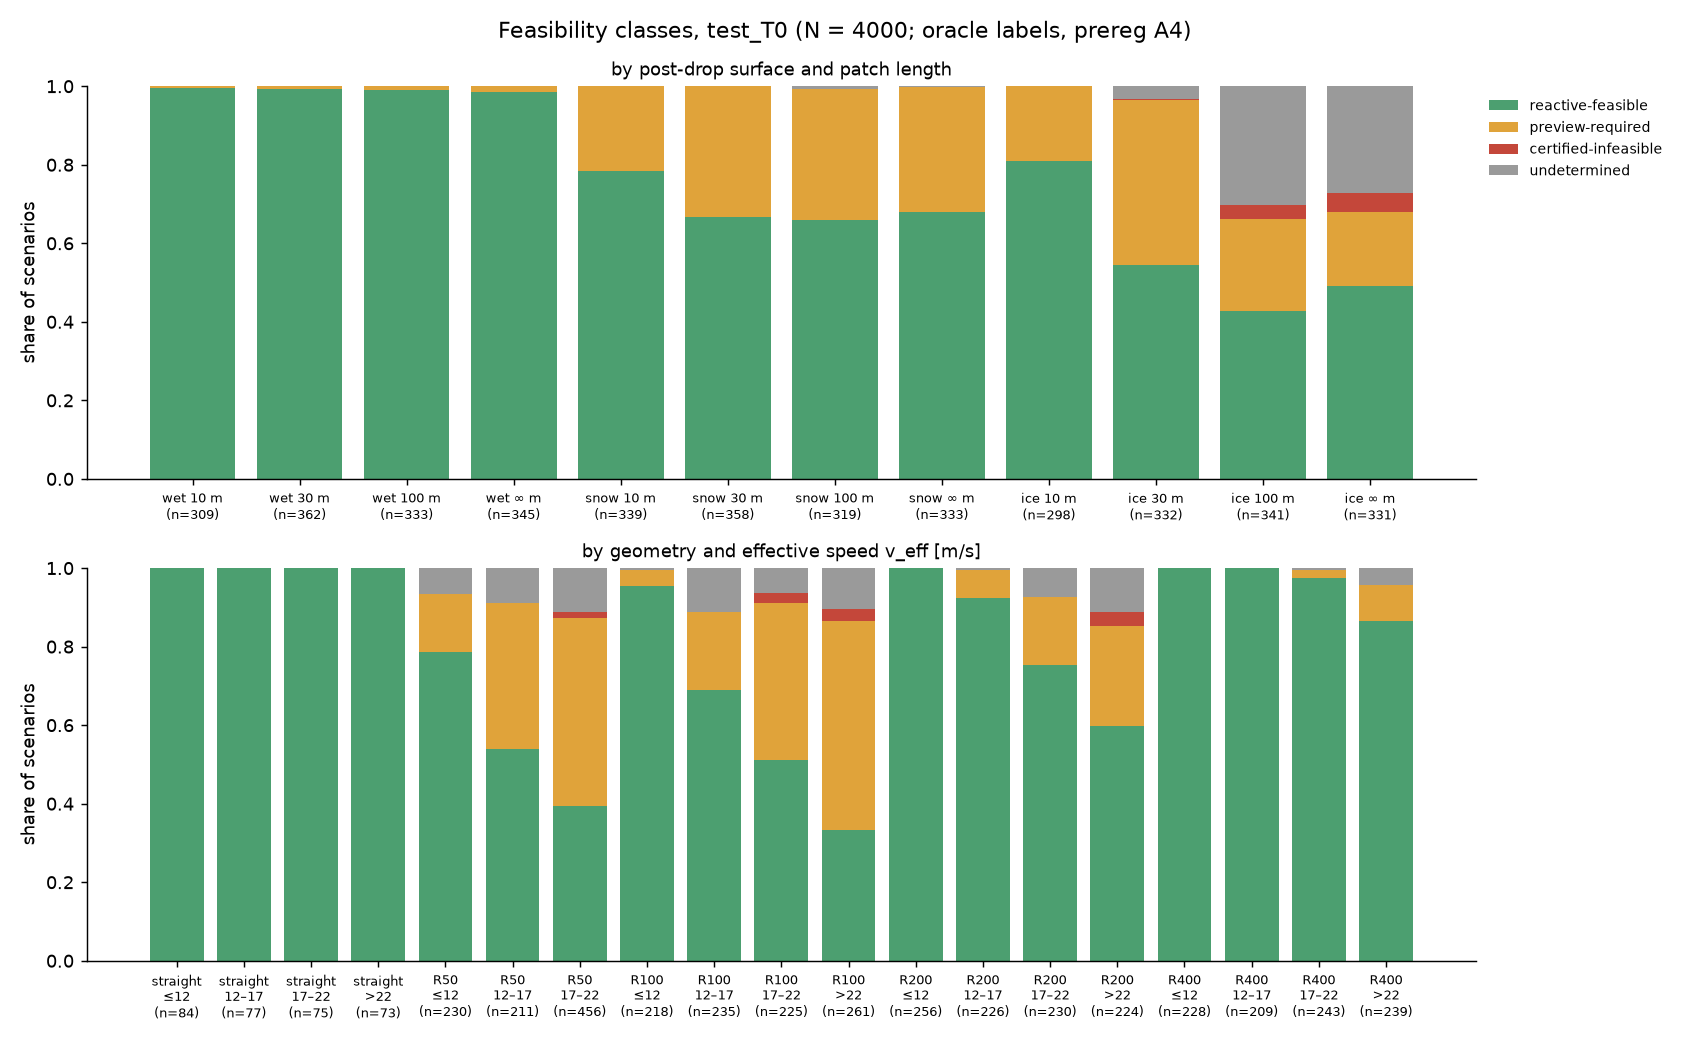
\includegraphics[width=\linewidth]{labels_test_T0.png}
\caption{Feasibility classes of the 4,000-scenario test pool by post-drop surface and patch length (top) and by
geometry and effective speed (bottom). Labels were produced with the frozen oracle settings before any method was
run on a test scenario.}
\label{fig:labels}
\end{figure}
\IfGen{gen/labels.tex}{label counts}

\section{Methods compared}\label{sec:methods}
\begin{center}\small
\begin{tabular}{@{}llll@{}}
\toprule
ID & Controller & Friction information & Role\\
\midrule
O-R & reactive-oracle MPPI & true current per-axle $\mu$ & regret reference\\
O-C & clairvoyant-oracle MPPI & true $\mu$ map ahead & labelling only\\
M-N & nominal MPPI & assumes dry & context\\
M-B & bank-adaptive MPPI & model with least look-back error & adaptive baseline\\
M-L & learned-estimator MPPI & GRU estimate from history & adaptive baseline\\
P-T & PPO teacher & privileged current $\mu$ & policy upper bound\\
\textbf{P-S} & \textbf{RMA student} & latent regressed from history & \textbf{method under test}\\
P-DR & domain-randomised PPO & none & robustness baseline\\
P-SP & student of a 30\,m-preview teacher & none (teacher had preview) & H3 ablation\\
\bottomrule
\end{tabular}
\end{center}
\textbf{Matched information.} Every adaptive method (M-B, M-L, P-S, P-SP) sees the same noisy observation channels
(IMU, wheel speeds, steering angle, last actions, path-relative state and the geometry ahead, never the friction
ahead) over the same history window. \textbf{Matched effort.} Each tunable method gets 20 Optuna TPE trials and
15 GPU-hours on the tuning split, whichever binds first; the student's budget includes its teacher's trials and
M-L's includes estimator training. The ledger of every trial and GPU-second is part of the repository.
The bank covers the same friction and extra-delay range as the RL domain randomisation.

\section{Pre-registered protocol}\label{sec:protocol}
\textbf{H1} (RQ1): on reactive-feasible scenarios, P-S's lane-departure rate is not lower than the better of M-B/M-L
by more than 5 percentage points. Falsified if the paired difference (better MPPI $-$ P-S) has a 95\% CI entirely
above $+5$\,pp. \textbf{H2} (RQ2): as the truth leaves the nominal model family along three axes (combined-slip
formulation, tire relaxation length, extra actuator delay up to +140\,ms; all outside the DR support and the bank),
adaptive-MPPI regret against O-R grows faster than the student's. \textbf{H3} (RQ3): the current-friction student
matches or beats the preview-teacher student on departure without a dry-pace cost of 2\% or more.
Statistics: hierarchical bootstrap over scenarios and seeds, TOST at $\pm5$\,pp, Holm--Bonferroni over H1--H3.
The protocol was tagged \texttt{prereg-v1} before any test scenario was labelled; six dated amendments (A1--A6)
record later decisions, each before the data it concerns. Amendment A6, for instance, was triggered by a pipeline
dry run on tuning data: at +140\,ms delay the shared driver itself can fail to reach the handover state, and such
scenarios are excluded from every level of that axis for every method.

\section{Implementation}\label{sec:impl}
The simulator, reference MPPI, RL environment and PPO run on one GPU (RTX 5090 Laptop) through zero-copy
Warp/PyTorch tensors. The C++17/CUDA MPPI shares one \texttt{\_\_host\_\_ \_\_device\_\_} source between a CPU and a CUDA
driver, exposes a C ABI used from Python through ctypes on device pointers, and is tested with GoogleTest (CPU and
CUDA) in CI. It reproduces Warp's random number generator bit for bit, so both implementations draw identical
samples. Gate S3 compares whole control steps from 1,000 perturbed states. The remaining differences come from
compiler-dependent fused multiply-add placement, so confirmatory runs use one backend throughout.
\IfGen{gen/compute.tex}{compute and latency table}

\section{Results}\label{sec:results}
\IfGen{gen/results.tex}{confirmatory results H1--H3 with N and 95\% CIs; per-class departure; regime map; mechanism}

\section{Grounding against real driving data}\label{sec:grounding}
The simulator's steady-state cornering response is compared with openpilot-engaged driving of ten passenger-car
platforms in the commaSteeringControl dataset~\citep{comma}. The understeer gradient is fitted with the steering
ratio left free, so only the wheelbase is taken from the car specifications.
\IfGen{gen/grounding.tex}{understeer comparison}

\section{Limitations}
Simulation only: a planar single-track model without roll or lateral load transfer, one vehicle, friction that
changes along the lane only, and labels that hold for this model. The oracles are strong but finite witnesses, so the
undetermined class is reported separately. All training, tuning and evaluation run on a single laptop GPU, which
bounds the scenario counts and the number of training seeds.

\bibliographystyle{plainnat}
\bibliography{refs}
\end{document}
